\documentclass[12pt,a4paper]{article}

% ============================================================
% CONFIGURACIÓN GENERAL
% ============================================================

\usepackage[spanish,es-tabla,es-nodecimaldot]{babel}
\usepackage[utf8]{inputenc}
\usepackage[T1]{fontenc}
\usepackage{lmodern}
\usepackage{microtype}

\usepackage[a4paper,margin=2.5cm]{geometry}
\usepackage{setspace}
\onehalfspacing

\usepackage{amsmath,amssymb,mathtools}
\usepackage{siunitx}
\sisetup{
    output-decimal-marker = {,},
    group-separator = {.},
    group-digits = integer,
    group-minimum-digits = 4
}

\usepackage{graphicx}
\usepackage{float}
\usepackage{caption}
\usepackage{subcaption}

\usepackage{booktabs}
\usepackage{array}
\usepackage{longtable}
\usepackage{multirow}

\usepackage{xcolor}
\usepackage[most]{tcolorbox}
\usepackage{fancyhdr}
\usepackage{lastpage}
\usepackage{hyperref}
\usepackage{xurl}

\hypersetup{
    colorlinks=true,
    linkcolor=black,
    urlcolor=blue,
    citecolor=black
}

% ============================================================
% COLORES Y CAJAS
% ============================================================

\definecolor{utnblue}{HTML}{003A70}
\definecolor{softblue}{HTML}{EAF3FF}
\definecolor{softgray}{HTML}{F5F5F5}
\definecolor{darkgray}{HTML}{333333}

\newtcolorbox{importantbox}{
    colback=softblue,
    colframe=utnblue,
    arc=2mm,
    boxrule=0.8pt,
    left=2mm,
    right=2mm,
    top=1mm,
    bottom=1mm
}

\newtcolorbox{methodbox}{
    colback=softgray,
    colframe=darkgray,
    arc=2mm,
    boxrule=0.6pt,
    left=2mm,
    right=2mm,
    top=1mm,
    bottom=1mm
}

% ============================================================
% ENCABEZADO Y PIE
% ============================================================

\pagestyle{fancy}
\fancyhf{}
\lhead{Análisis Numérico}
\rhead{Aproximación discreta}
\cfoot{\thepage\ de \pageref{LastPage}}

% ============================================================
% COMANDOS ÚTILES
% ============================================================

\newcommand{\temperatura}{T}
\newcommand{\demanda}{D}
\newcommand{\unidadDemanda}{\text{MM m}^3/\text{día}}
\newcommand{\unidadTemp}{^\circ\text{C}}

\newcommand{\modeloLineal}{f_1(T)=a+bT}
\newcommand{\modeloCuadratico}{f_2(T)=a+bT+cT^2}
\newcommand{\modeloExponencial}{f_3(T)=Ae^{BT}}

% ============================================================
% DATOS DEL TRABAJO
% ============================================================

\title{
    \vspace{-1cm}
    \textbf{\Large Aproximación discreta por mínimos cuadrados}\\[0.3cm]
    \large Demanda prioritaria de gas natural en función de la temperatura media
}

\author{
\begin{tabular}{ll}
Alex Fiorenza & \href{mailto:afiorenza@frba.utn.edu.ar}{afiorenza@frba.utn.edu.ar}\\
Valentina Veron & \href{mailto:vveron@frba.utn.edu.ar}{vveron@frba.utn.edu.ar}\\
Juan Francisco Aldaco & \href{mailto:jaldaco@frba.utn.edu.ar}{jaldaco@frba.utn.edu.ar}\\
Francisco Fernando Garcia & \href{mailto:frgarcia@frba.utn.edu.ar}{frgarcia@frba.utn.edu.ar}\\
Franco Uriel Schendel & \href{mailto:fschendel@frba.utn.edu.ar}{fschendel@frba.utn.edu.ar}\\
Felipe Fernández Presedo & \href{mailto:ffernandezpresedo@frba.utn.edu.ar}{ffernandezpresedo@frba.utn.edu.ar}
\end{tabular}
}

\date{
    Universidad Tecnológica Nacional -- Facultad Regional Buenos Aires\\
    Análisis Numérico\\
    \today
}

\begin{document}

\maketitle

\begin{abstract}
En este trabajo se aplica el método de mínimos cuadrados a un conjunto de datos discretos reales para estudiar la relación entre la temperatura media diaria y la demanda prioritaria de gas natural. Se ajustan tres modelos: lineal, cuadrático y exponencial. El modelo exponencial se incorpora como modelo no polinómico y se resuelve mediante una transformación logarítmica. Luego se comparan los modelos mediante métricas de error y se utiliza el modelo seleccionado para estimar la demanda correspondiente a una temperatura media dada.
\end{abstract}

\begin{importantbox}
\textbf{Nota metodológica.} La fuente de ENARGAS publica valores de demanda prioritaria, algunos de los cuales pueden corresponder a estimaciones operativas. En este trabajo no se pretende reproducir el modelo oficial de ENARGAS, sino construir una aproximación matemática simplificada mediante mínimos cuadrados, utilizando la temperatura media como variable explicativa.
\end{importantbox}

\tableofcontents
\newpage

% ============================================================
\section{Introducción}

La demanda de gas natural presenta una relación directa con las condiciones climáticas. En particular, durante los días de menor temperatura suele observarse un mayor consumo debido al uso de calefacción en hogares, comercios e instituciones. Por este motivo, resulta razonable estudiar la demanda prioritaria de gas natural como función de la temperatura media diaria.

El objetivo de este trabajo es aplicar el método de mínimos cuadrados para aproximar datos discretos reales mediante distintos modelos funcionales. Se consideran tres modelos: uno lineal, uno cuadrático y uno exponencial. Finalmente, se comparan los resultados y se selecciona el modelo más adecuado para estimar la demanda correspondiente a una temperatura media determinada.

% ============================================================
\section{Descripción del problema}

Se trabaja con dos variables:

\begin{itemize}
    \item Variable independiente:
    \[
        x_i = T_i
    \]
    donde \(T_i\) representa la temperatura media diaria, medida en grados Celsius.

    \item Variable dependiente:
    \[
        y_i = D_i
    \]
    donde \(D_i\) representa la demanda prioritaria de gas natural, medida en \(\unidadDemanda\).
\end{itemize}

El conjunto de datos queda formado por pares discretos:

\[
(T_1,D_1), (T_2,D_2), \dots, (T_n,D_n)
\]

El problema consiste en encontrar una función aproximante:

\[
D \approx f(T)
\]

que permita estimar la demanda de gas natural para una temperatura media \(T_0\) que no se encuentra directamente observada en el conjunto de datos.

\begin{importantbox}
En este trabajo se estima la demanda para:
\[
    T_0 = \boxed{8} \ \unidadTemp
\]
Este valor debe pertenecer al intervalo de temperaturas observado para que la estimación corresponda a una interpolación.
\end{importantbox}

% ============================================================
\section{Fuente y preparación de los datos}

Los datos de demanda provienen de registros publicados por ENARGAS. El archivo utilizado contiene las columnas:

\begin{center}
\texttt{fecha}, \texttt{licenciataria}, \texttt{demanda\_millones\_m3d}
\end{center}

A partir de estos registros, se agrupa la demanda por fecha y se define la variable dependiente. Para mantener coherencia geográfica con la temperatura media del Gran Buenos Aires, se propone utilizar:

\[
    D_{GBA} = D_{\text{MetroGAS}} + D_{\text{Naturgy BAN}}
\]

También podría utilizarse la demanda total nacional:

\[
    D_{\text{total}} = \sum_{\text{licenciatarias}} D_j
\]

aunque esta opción mezcla una variable climática local con una demanda territorialmente más amplia.

\begin{methodbox}
\textbf{Criterio adoptado.}
\[
    D_i = \boxed{D_{\text{MetroGAS}} + D_{\text{Naturgy BAN}}}
\]
Se suman las dos licenciatarias que abastecen el Área Metropolitana de Buenos Aires, por coherencia geográfica con la temperatura media empleada como variable explicativa. Solo se conservan las fechas en las que ambas licenciatarias registran demanda.
\end{methodbox}

La temperatura media diaria se incorpora desde una segunda fuente de datos meteorológicos. En caso de contar con temperatura máxima y mínima diaria, se calcula:

\[
    T_{\text{media}} = \frac{T_{\max} + T_{\min}}{2}
\]

La temperatura media diaria de cada estación se calcula según la expresión anterior, a partir del registro diario del Servicio Meteorológico Nacional. Para obtener un valor representativo del Gran Buenos Aires, se promedió dicha temperatura media sobre las principales estaciones del Área Metropolitana (Aeroparque, Observatorio Central de Buenos Aires, Ezeiza, El Palomar, Morón, San Fernando, Campo de Mayo y La Plata). Finalmente, se unen ambos conjuntos por fecha, conservando únicamente los días con registros completos en ambas fuentes.

% ============================================================
\section{Tabla de datos}

La Tabla~\ref{tab:datos-muestra} muestra una muestra del conjunto de datos final utilizado para el ajuste.

\begin{table}[H]
\centering
\caption{Muestra de datos utilizados para el ajuste}
\label{tab:datos-muestra}
\begin{tabular}{l r r}
\toprule
Fecha & $T_i$ ($^\circ$C) & $D_i$ (MM m$^3$/día) \\
\midrule
2025-06-15 & \num{7.75} & \num{22.95} \\
2025-07-17 & \num{8.12} & \num{26.48} \\
2025-08-18 & \num{14.00} & \num{20.91} \\
2025-09-18 & \num{19.44} & \num{9.57} \\
2025-10-20 & \num{18.84} & \num{8.19} \\
2025-11-21 & \num{16.09} & \num{9.19} \\
2025-12-23 & \num{25.79} & \num{5.22} \\
2026-01-24 & \num{27.14} & \num{5.02} \\
2026-02-25 & \num{19.53} & \num{6.74} \\
2026-03-28 & \num{23.04} & \num{6.69} \\
2026-04-29 & \num{17.34} & \num{12.26} \\
2026-05-31 & \num{10.82} & \num{18.74} \\
\bottomrule
\end{tabular}

\end{table}

El conjunto completo contiene:

\[
    n = \boxed{351}
\]

observaciones válidas.

% ============================================================
\section{Nube de puntos}

Antes de ajustar los modelos se grafica la nube de puntos correspondiente a los pares observados \((T_i,D_i)\).

\begin{figure}[H]
\centering
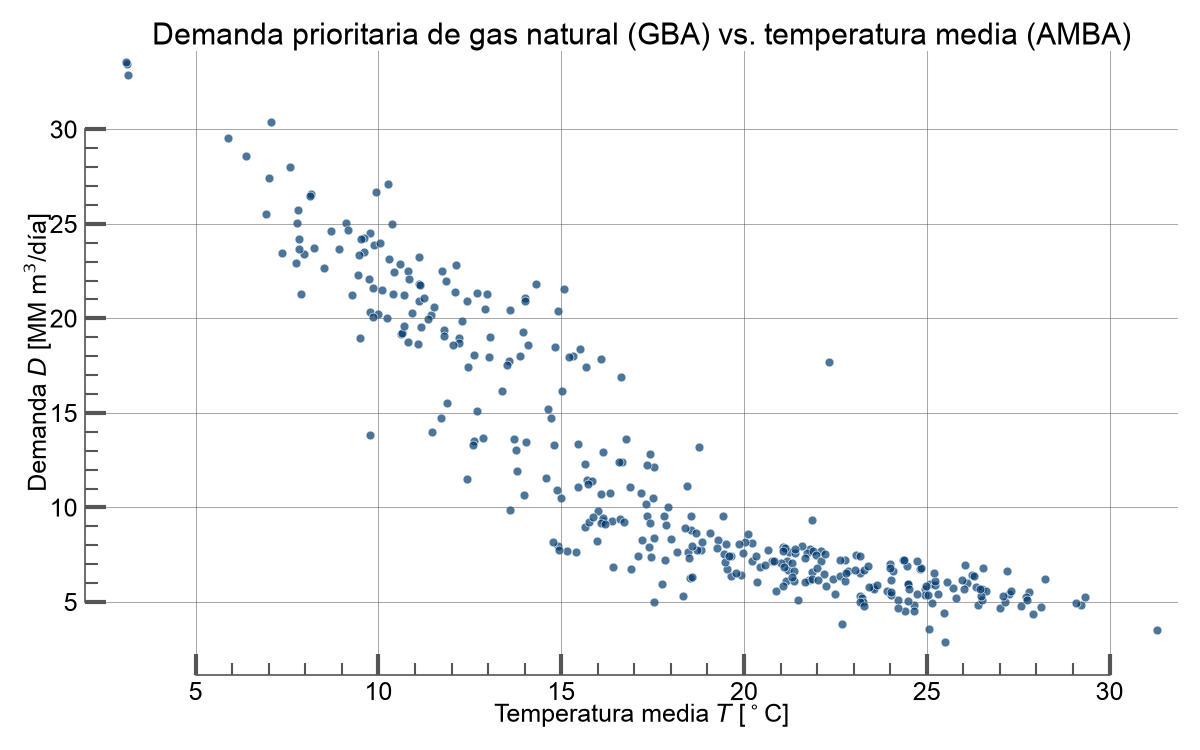
\includegraphics[width=0.82\textwidth]{figures/nube_puntos.png}
\caption{Nube de puntos: demanda prioritaria de gas natural en función de la temperatura media.}
\label{fig:nube}
\end{figure}

A partir de la Figura~\ref{fig:nube}, se espera observar una relación decreciente: a menor temperatura media, mayor demanda de gas natural.

% ============================================================
\section{Modelo lineal}

El primer modelo considerado es lineal:

\[
    \modeloLineal
\]

Se busca minimizar la suma de cuadrados de los errores:

\[
    S(a,b)=\sum_{i=1}^{n}\left[D_i-(a+bT_i)\right]^2
\]

Para obtener los coeficientes, se imponen las condiciones:

\[
    \frac{\partial S}{\partial a}=0,
    \qquad
    \frac{\partial S}{\partial b}=0
\]

De allí se obtiene el sistema de ecuaciones normales:

\[
\begin{cases}
na + b\sum T_i = \sum D_i \\
a\sum T_i + b\sum T_i^2 = \sum T_iD_i
\end{cases}
\]

En forma matricial:

\[
\begin{bmatrix}
n & \sum T_i \\
\sum T_i & \sum T_i^2
\end{bmatrix}
\begin{bmatrix}
a \\
b
\end{bmatrix}
=
\begin{bmatrix}
\sum D_i \\
\sum T_iD_i
\end{bmatrix}
\]

\subsection{Sustitución numérica}

\begin{table}[H]
\centering
\caption{Sumas utilizadas en el ajuste lineal}
\begin{tabular}{l r}
\toprule
Cantidad & Valor \\
\midrule
$n$ & \num{351} \\
$\sum T_i$ & \num{6250.89} \\
$\sum T_i^2$ & \num{123882.34} \\
$\sum D_i$ & \num{4213.72} \\
$\sum T_i D_i$ & \num{61546.62} \\
\bottomrule
\end{tabular}

\end{table}

El sistema resultante es:

\[
\begin{bmatrix}
\num{351} & \num{6250.89} \\
\num{6250.89} & \num{123882.34}
\end{bmatrix}
\begin{bmatrix}
a \\
b
\end{bmatrix}
=
\begin{bmatrix}
\num{4213.72} \\
\num{61546.62}
\end{bmatrix}
\]

Resolviendo:

\[
    a = \boxed{\num{31.1364}},
    \qquad
    b = \boxed{\num{-1.0743}}
\]

Por lo tanto, la función lineal aproximante queda:

\[
    f_1(T)=\boxed{\num{31.1364} - \num{1.0743}\,T}
\]

\begin{figure}[H]
\centering
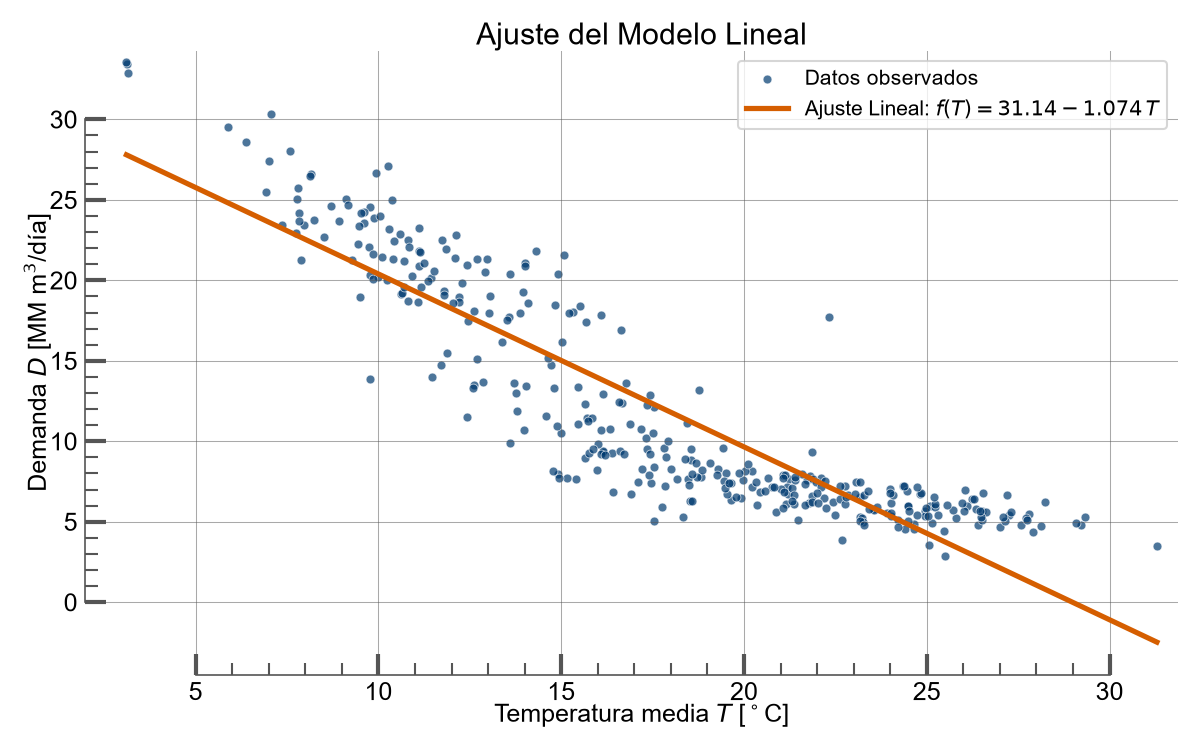
\includegraphics[width=0.88\textwidth]{figures/modelo_lineal.png}
\caption{Gráfica del modelo lineal ajustado sobre la nube de puntos.}
\label{fig:modelo_lineal}
\end{figure}

% ============================================================
\section{Modelo cuadrático}

El segundo modelo considerado es un polinomio de segundo grado:

\[
    \modeloCuadratico
\]

Se minimiza:

\[
    S(a,b,c)=\sum_{i=1}^{n}\left[D_i-(a+bT_i+cT_i^2)\right]^2
\]

Las ecuaciones normales son:

\[
\begin{cases}
na + b\sum T_i + c\sum T_i^2 = \sum D_i \\
a\sum T_i + b\sum T_i^2 + c\sum T_i^3 = \sum T_iD_i \\
a\sum T_i^2 + b\sum T_i^3 + c\sum T_i^4 = \sum T_i^2D_i
\end{cases}
\]

En forma matricial:

\[
\begin{bmatrix}
n & \sum T_i & \sum T_i^2 \\
\sum T_i & \sum T_i^2 & \sum T_i^3 \\
\sum T_i^2 & \sum T_i^3 & \sum T_i^4
\end{bmatrix}
\begin{bmatrix}
a \\
b \\
c
\end{bmatrix}
=
\begin{bmatrix}
\sum D_i \\
\sum T_iD_i \\
\sum T_i^2D_i
\end{bmatrix}
\]

\subsection{Sustitución numérica}

\begin{table}[H]
\centering
\caption{Sumas utilizadas en el ajuste cuadrático}
\begin{tabular}{l r}
\toprule
Cantidad & Valor \\
\midrule
$n$ & \num{351} \\
$\sum T_i$ & \num{6250.89} \\
$\sum T_i^2$ & \num{123882.34} \\
$\sum T_i^3$ & \num{2644334.76} \\
$\sum T_i^4$ & \num{59479524.45} \\
$\sum D_i$ & \num{4213.72} \\
$\sum T_i D_i$ & \num{61546.62} \\
$\sum T_i^2 D_i$ & \num{1041768.03} \\
\bottomrule
\end{tabular}

\end{table}

El sistema resultante es:

\[
\begin{bmatrix}
\num{351} & \num{6250.89} & \num{123882.34} \\
\num{6250.89} & \num{123882.34} & \num{2644334.76} \\
\num{123882.34} & \num{2644334.76} & \num{59479524.45}
\end{bmatrix}
\begin{bmatrix}
a \\
b \\
c
\end{bmatrix}
=
\begin{bmatrix}
\num{4213.72} \\
\num{61546.62} \\
\num{1041768.03}
\end{bmatrix}
\]

Resolviendo:

\[
    a = \boxed{\num{45.4180}},
    \qquad
    b = \boxed{\num{-2.9315}},
    \qquad
    c = \boxed{\num{0.05325}}
\]

Por lo tanto, la función cuadrática aproximante queda:

\[
    f_2(T)=\boxed{\num{45.4180} - \num{2.9315}\,T + \num{0.05325}\,T^2}
\]

\begin{figure}[H]
\centering
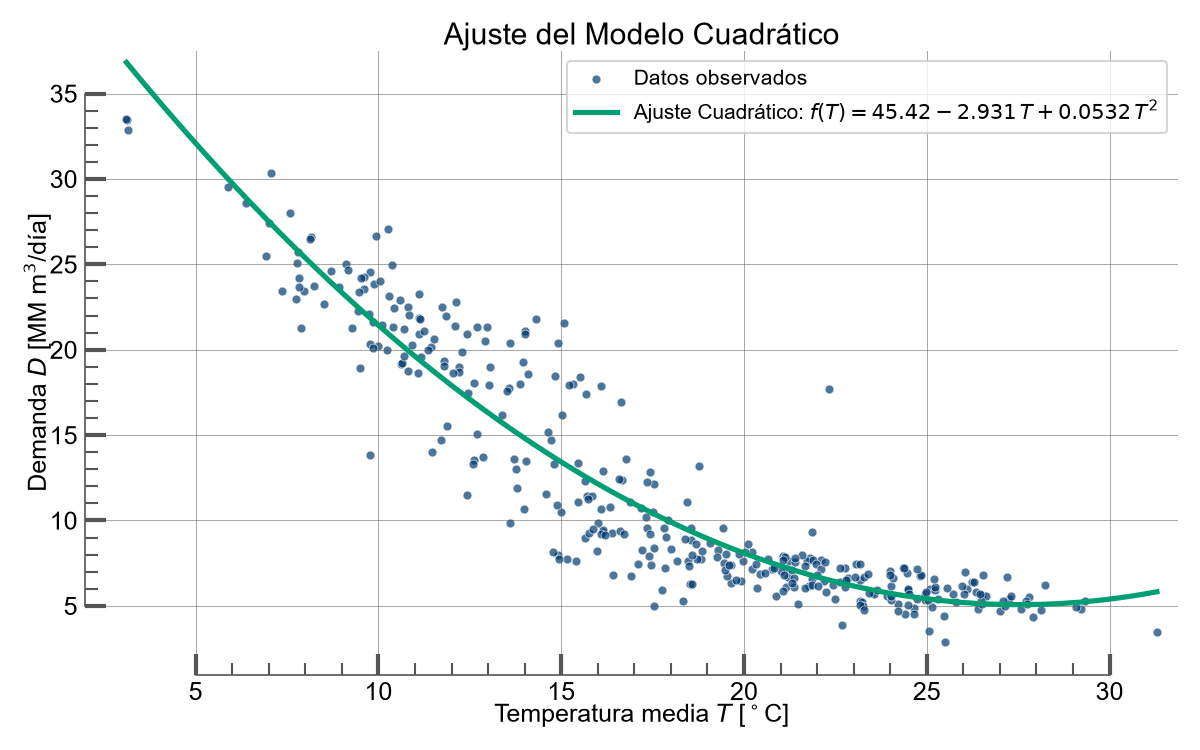
\includegraphics[width=0.88\textwidth]{figures/modelo_cuadratico.png}
\caption{Gráfica del modelo cuadrático ajustado sobre la nube de puntos.}
\label{fig:modelo_cuadratico}
\end{figure}

% ============================================================
\section{Modelo exponencial}

El tercer modelo considerado es no polinómico:

\[
    \modeloExponencial
\]

Como el modelo no es lineal en sus parámetros, se aplica logaritmo natural:

\[
    D = Ae^{BT}
\]

\[
    \ln(D)=\ln(Ae^{BT})
\]

\[
    \ln(D)=\ln(A)+BT
\]

Definimos:

\[
    Y = \ln(D),
    \qquad
    \alpha = \ln(A)
\]

Entonces:

\[
    Y = \alpha + BT
\]

El ajuste se reduce a un modelo lineal sobre los datos transformados \((T_i,Y_i)\), donde:

\[
    Y_i = \ln(D_i)
\]

Las ecuaciones normales son:

\[
\begin{cases}
n\alpha + B\sum T_i = \sum Y_i \\
\alpha\sum T_i + B\sum T_i^2 = \sum T_iY_i
\end{cases}
\]

En forma matricial:

\[
\begin{bmatrix}
n & \sum T_i \\
\sum T_i & \sum T_i^2
\end{bmatrix}
\begin{bmatrix}
\alpha \\
B
\end{bmatrix}
=
\begin{bmatrix}
\sum Y_i \\
\sum T_iY_i
\end{bmatrix}
\]

\subsection{Sustitución numérica}

\begin{table}[H]
\centering
\caption{Sumas utilizadas en el ajuste exponencial}
\begin{tabular}{l r}
\toprule
Cantidad & Valor \\
\midrule
$n$ & \num{351} \\
$\sum T_i$ & \num{6250.89} \\
$\sum T_i^2$ & \num{123882.34} \\
$\sum Y_i$ & \num{814.2272} \\
$\sum T_i Y_i$ & \num{13397.9888} \\
\bottomrule
\end{tabular}

% Y_i = ln(D_i)

\end{table}

Resolviendo:

\[
    \alpha = \boxed{\num{3.8827}},
    \qquad
    B = \boxed{\num{-0.08776}}
\]

Luego:

\[
    A = e^{\alpha}
\]

Por lo tanto:

\[
    A = \boxed{\num{48.5527}}
\]

y la función exponencial aproximante queda:

\[
    f_3(T)=\boxed{\num{48.5527}\,e^{\num{-0.08776}\,T}}
\]

\begin{figure}[H]
\centering
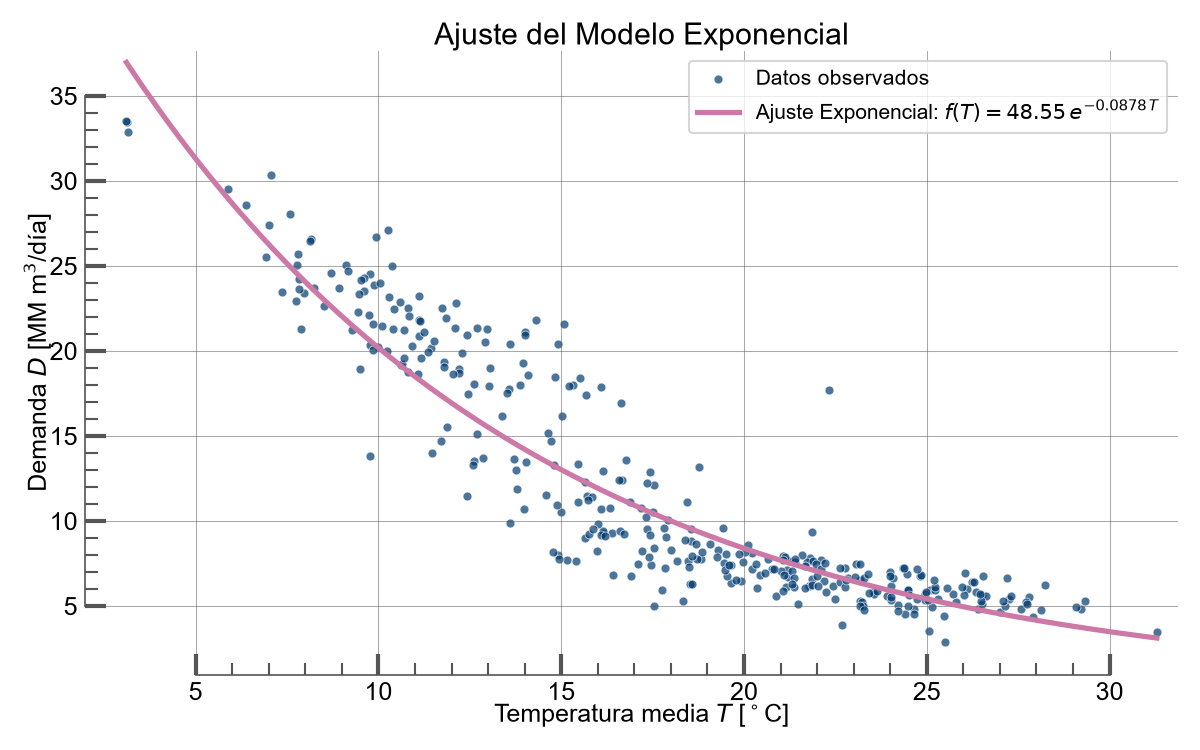
\includegraphics[width=0.88\textwidth]{figures/modelo_exponencial.png}
\caption{Gráfica del modelo exponencial ajustado sobre la nube de puntos.}
\label{fig:modelo_exponencial}
\end{figure}

% ============================================================
\section{Comparación de modelos}

Para comparar los modelos se calculan los residuos:

\[
    r_i = D_i - f(T_i)
\]

También se utilizan las siguientes métricas:

\[
    SSE = \sum_{i=1}^{n} \left(D_i-f(T_i)\right)^2
\]

\[
    RMSE = \sqrt{\frac{1}{n}\sum_{i=1}^{n} \left(D_i-f(T_i)\right)^2}
\]

\[
    R^2 = 1 - \frac{\sum_{i=1}^{n}(D_i-f(T_i))^2}
    {\sum_{i=1}^{n}(D_i-\overline{D})^2}
\]

donde:

\[
    \overline{D} = \frac{1}{n}\sum_{i=1}^{n}D_i
\]

\begin{table}[H]
\centering
\caption{Coeficientes de los modelos ajustados}
\label{tab:coeficientes}
\begin{tabular}{l l}
\toprule
Modelo & Función ajustada \\
\midrule
Lineal & $f_1(T)=\num{31.1364} - \num{1.0743}\,T$ \\
Cuadrático & $f_2(T)=\num{45.4180} - \num{2.9315}\,T + \num{0.05325}\,T^2$ \\
Exponencial & $f_3(T)=\num{48.5527}\,e^{\num{-0.08776}\,T}$ \\
\bottomrule
\end{tabular}

\end{table}

\begin{table}[H]
\centering
\caption{Comparación de métricas de error}
\label{tab:metricas}
\begin{tabular}{l r r r}
\toprule
Modelo & SSE & RMSE & $R^2$ \\
\midrule
Lineal & \num{3384.59} & \num{3.1053} & \num{0.8107} \\
Cuadrático\;$\star$ & \num{2039.79} & \num{2.4107} & \num{0.8859} \\
Exponencial & \num{2315.97} & \num{2.5687} & \num{0.8705} \\
\bottomrule
\end{tabular}

% El modelo marcado con $\star$ es el seleccionado (menor RMSE).

\end{table}

\begin{figure}[H]
\centering
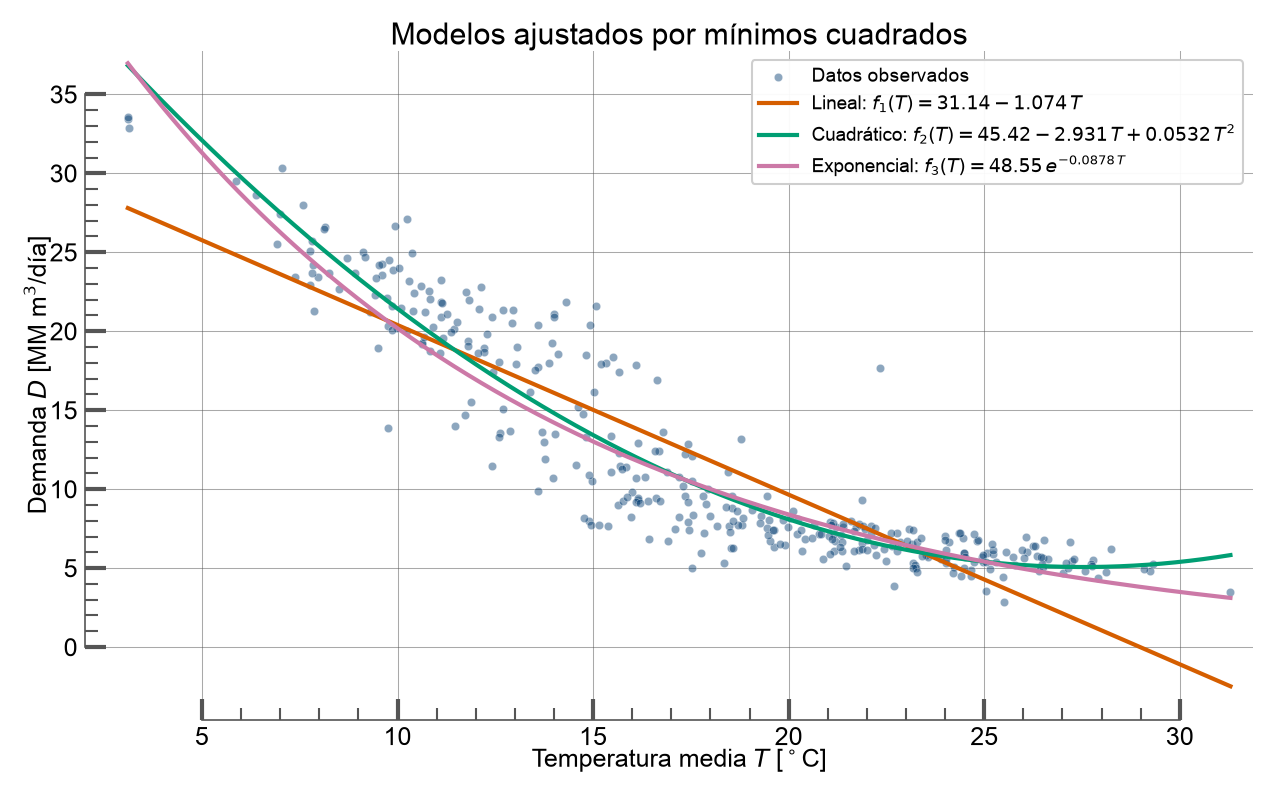
\includegraphics[width=0.88\textwidth]{figures/modelos_ajustados.png}
\caption{Comparación de los tres modelos ajustados sobre la nube de puntos.}
\label{fig:modelos}
\end{figure}

\begin{figure}[H]
\centering
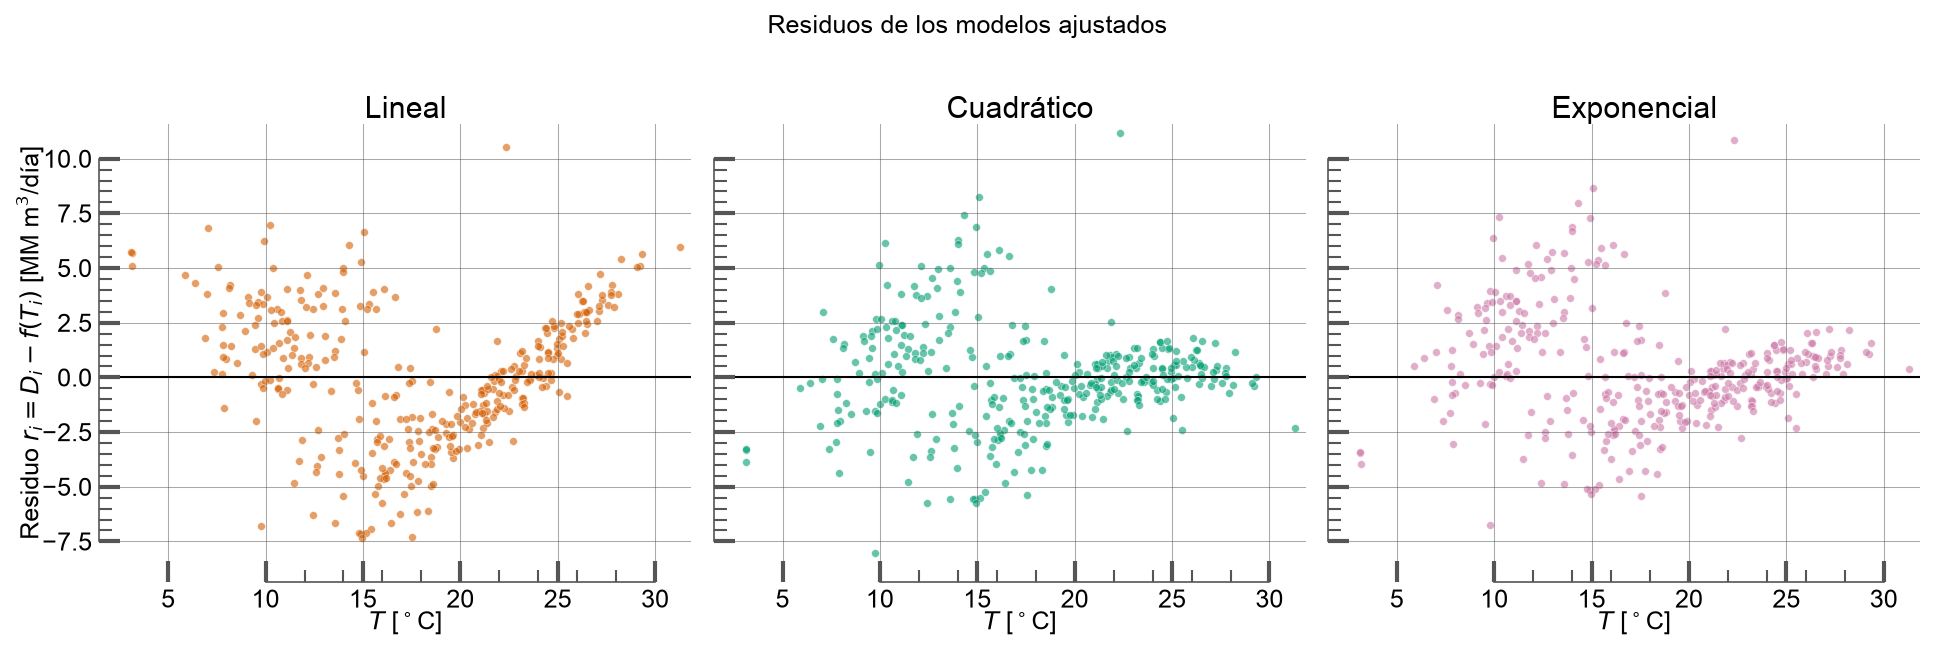
\includegraphics[width=0.88\textwidth]{figures/residuos.png}
\caption{Residuos de los modelos ajustados.}
\label{fig:residuos}
\end{figure}

A partir de las métricas obtenidas, el modelo seleccionado es:

\[
    \boxed{\text{Modelo cuadrático:}\quad f_2(T)=a+bT+cT^2}
\]

El criterio de selección utilizado fue el menor \(RMSE\), junto con la coherencia del modelo respecto del fenómeno observado.

Los tres modelos reproducen la relación decreciente entre demanda y temperatura, pero el modelo lineal presenta residuos con un patrón sistemático en forma de \(U\) (Figura~\ref{fig:residuos}), lo que evidencia que la relación no es lineal. El modelo cuadrático obtiene el menor \(RMSE\) y el mayor \(R^2\), por lo que se lo adopta como modelo seleccionado. No obstante, conviene señalar que el modelo exponencial, con métricas muy próximas, resulta más coherente para valores extremos de temperatura: es siempre positivo y monótono decreciente, mientras que el polinomio cuadrático presenta una leve curvatura ascendente para temperaturas altas (Figura~\ref{fig:modelos}) que carece de sentido físico. Dado que la estimación pedida corresponde a \(T_0 = 8\,\unidadTemp\), ubicada en la zona donde ambos modelos prácticamente coinciden y se ajustan muy bien a los datos, se utiliza el modelo cuadrático.

% ============================================================
\section{Estimación del valor pedido}

Se desea estimar la demanda prioritaria de gas natural para:

\[
    T_0 = \boxed{8} \ \unidadTemp
\]

Utilizando el modelo seleccionado:

\[
    D(T_0)=f(T_0)
\]

\begin{table}[H]
\centering
\caption{Estimación final}
\label{tab:estimacion-final}
\begin{tabular}{l r}
\toprule
Concepto & Valor \\
\midrule
Modelo seleccionado & Cuadrático \\
$T_0$ & \num{8} $^\circ$C \\
$D(T_0)$ & \num{25.37} MM m$^3$/día \\
\bottomrule
\end{tabular}

\end{table}

Por lo tanto, la demanda estimada para una temperatura media de \(T_0\) es:

\[
    \boxed{D(T_0)=\num{25.37} \ \unidadDemanda}
\]

% ============================================================
\section{Análisis de confiabilidad}

Para analizar la confiabilidad de la estimación se verifica si \(T_0\) pertenece al rango de temperaturas observado:

\[
    T_{\min} \leq T_0 \leq T_{\max}
\]

Si esta condición se cumple, la estimación corresponde a una interpolación. En cambio, si \(T_0\) se encuentra fuera del rango observado, el cálculo corresponde a una extrapolación y resulta menos confiable.

Además, se consideran los residuos y las métricas de error del modelo elegido. Un menor \(RMSE\) indica que, en promedio, las predicciones se encuentran más cerca de los valores observados. Sin embargo, debe tenerse en cuenta que la demanda de gas natural no depende únicamente de la temperatura: también intervienen factores como día de la semana, estacionalidad, actividad económica, feriados, comportamiento residencial y condiciones operativas del sistema.

% ============================================================
\section{Conclusiones}

En este trabajo se aplicó el método de mínimos cuadrados para aproximar la demanda prioritaria de gas natural en función de la temperatura media diaria. Se utilizaron datos discretos reales y se ajustaron tres modelos:

\begin{itemize}
    \item modelo lineal;
    \item modelo cuadrático;
    \item modelo exponencial.
\end{itemize}

El modelo exponencial permitió cumplir con el requisito de incorporar un modelo no polinómico, resolviéndose mediante una transformación logarítmica.

Luego de comparar las métricas de error, se seleccionó el modelo:

\[
    \boxed{\text{Modelo cuadrático:}\quad f_2(T)=a+bT+cT^2}
\]

Con dicho modelo se estimó la demanda correspondiente a:

\[
    T_0 = \boxed{8} \ \unidadTemp
\]

obteniendo:

\[
    D(T_0)=\boxed{\num{25.37}} \ \unidadDemanda
\]

La confiabilidad de esta estimación depende de que \(T_0\) se encuentre dentro del rango observado y de que los residuos del modelo no presenten patrones sistemáticos significativos.

% ============================================================
\section{Bibliografía}

\begin{itemize}
    \item ENARGAS. Estimación de la Demanda Prioritaria.\\
    \url{https://www.enargas.gob.ar/secciones/transporte-y-distribucion/dod-estimacion-demanda-prioritaria.php}

    \item ENARGAS. Datos históricos de demanda prioritaria.\\
    \url{https://www.enargas.gob.ar/secciones/transporte-y-distribucion/estimacion-demanda-prioritaria/estimacion_demanda_prioritaria.csv}

    \item Datos Argentina. Partes diarios de gas natural.\\
    \url{https://datos.gob.ar/ar/dataset/energia-partes-diarios-gas-natural}

    \item Servicio Meteorológico Nacional. Datos meteorológicos y registros de temperatura.\\
    \url{https://datos.gob.ar/dataset/smn-datos-meteorologicos-horarios}
\end{itemize}

\end{document}
